\documentclass{article}

% Language setting
% Replace `english' with e.g. `spanish' to change the document language
\usepackage[english]{babel}

% Set page size and margins
% Replace `letterpaper' with `a4paper' for UK/EU standard size
\usepackage[letterpaper,top=2cm,bottom=2cm,left=3cm,right=3cm,marginparwidth=1.75cm]{geometry}

% Useful packages
\usepackage{fancyhdr}
\usepackage{amsmath}
\usepackage{graphicx}
\usepackage[colorlinks=true, allcolors=blue]{hyperref}
\usepackage{titlesec}
\usepackage{enumitem}
\usepackage{amssymb}
\usepackage{amsthm}
\usepackage{tikz}
\usepackage{pgfplots}
\usepackage{float}
\usepackage{subcaption}
\usepackage{listings}
\usepackage{color}

\title{\vspace*{-3cm} % Adjusted to reduce the top margin
      \begin{center}
            \hspace*{0cm} % Adjusted to extend the black strip to the left
            \begin{tabular}{l@{}c@{}r}
                  \begin{tabular}{@{}c}
                        \textbf{Problem Chosen} \\
                        \textcolor{red}{\textbf{C}}
                  \end{tabular} &
                  \begin{tabular}{@{}c}
                      \textbf{2024} \\
                      \textbf{MCM/ICM} \\
                      \textbf{Summary Sheet}
                  \end{tabular} &
                  \begin{tabular}{@{}c}
                      \textcolor{black}{\textbf{Team control number}} \\
                      \textcolor{red}{\textbf{90169}}
                  \end{tabular}
            \end{tabular} \\[0.3cm]
            \rule{\linewidth}{2pt} % Adjust the width and height here
            \vspace{-2.5cm} % Adjusted to reduce the bottom margin
      \end{center}
}

\date{} % Removes the date
\author{} % Removes the author

\begin{document}
\maketitle
\section{Abstract}
My introduction goes here! Simply start writing your document and use the Recompile button to view the updated PDF preview. Examples of commonly used commands and features are listed below, to help you get started.
Once you're familiar with the editor, you can find various project settings in the Overleaf menu, accessed via the button in the very top left of the editor. To view tutorials, user guides, and further documentation, please visit our \href{https://www.overleaf.com/learn}{help library}, or head to our plans page to \href{https://www.overleaf.com/user/subscription/plans}{choose your plan}.

% Define header and footer
\pagestyle{fancy}
\fancyhf{} % Clear default header and footer
% Header
\fancyhead[C]{\textbf{Tennis Model}} % Centered header content
\fancyhead[L]{\textit{Team control number 90169}} % Left-aligned header content

% Footer
\fancyfoot[C]{\thepage} % Centered page number
\fancyfoot[L]{\textcolor{gray}{2024 MCM/ICM C 90169}} % Left-aligned footer content
\fancyfoot[R]{\textcolor{gray}{}} % Right-aligned footer content

\newpage
\tableofcontents % Table of contents
\newpage

\section{Introduction}
\subsection{Background}
Tennis originated in the 13th century in France. As early as the 16th to 17th centuries, French missionaries often played a game similar to tennis in the corridors of churches, using their hands to strike a small ball,
providing a diversion from the monotonous church life. Now, modern tennis has formally developed and quickly gained popularity in Europe and America, becoming a widely loved sport. [1] Tennis, as a charming and elegant sport, enjoys a high reputation and strong influence internationally. [2] With the continuous development of tennis, the fluctuations in the scores of opponents have become increasingly scrutinized during tennis matches. Recently, in the men's singles final at Wimbledon in 2023, 20-year-old Spanish rising star Carlos Alcaraz defeated 36-year-old Novak Djokovic, ending Djokovic's winning streak at Wimbledon since 2013. The twists and turns in the score and the changing dynamics of the match attracted significant attention. Therefore, effectively exploring the impact of the "momentum" on the score during the game is crucial.

\subsection{Problem restatement}
\begin{enumerate}
\item  Develop a mathematical model to quantify and visualize the progression of tennis matches, identifying key performance metrics for players during specific time intervals, with a particular focus on the service advantage.
\item Construct a statistical framework to assess the impact of momentum within a match, challenging the notion that players' swings in performance are random, and providing empirical evidence for or against this assertion.
\item Formulate a predictive model capable of indicating potential shifts in match dynamics, utilizing data from previous matches to identify indicators that signal when the flow of play may change in favor of one player over another.
\item Execute a comprehensive testing protocol for the aforementioned models across a series of matches, evaluating the predictive capabilities with respect to different match conditions, and identifying additional variables that may enhance future model iterations. Analyze the generalizability of the models to other match formats and sporting contexts, such as women's tennis, various tournaments, court surfaces, and racket sports akin to table tennis.
\end{enumerate}
\subsection{Our Work}
Tennis originated in the 13th century in France. As early as the 1st century, French missionaries often played with their hands in the corridors of churches, hitting a small ball-like
object to alleviate the monotonous church life. Now, modern tennis has formally developed and quickly gained popularity in Europe and America, becoming a widely loved sport. [1] Tennis, as a charming and elegant sport,
enjoys a high reputation and strong influence internationally. [2] With the continuous development of tennis, the fluctuations in scores and game situations during tennis matches have increasingly attracted people's attention.
Recently, in the men's singles final of the 2023 Wimbledon Championships, 20-year-old Spanish newcomer Carlos Alcaraz defeated 36-year-old Novak Djokovic, ending Djokovic's winning streak at Wimbledon since 2013. The twists and turns in the score
and the repeated changes in the game situation during the match have captured people's attention. Therefore, it is crucial to effectively explore the impact of "momentum" on the score during the course of the game.
\section{Symbol Description}
\begin{table}[H]
\centering
\begin{tabular}{|c|l|}
\hline
\textbf{Symbol} & \textbf{Description} \\ \hline
$S1$ & The number of game winning in the current set \\ \hline
$S2$ & The leading score in the current game \\ \hline
$S3$ & Whether it is the server \\ \hline
$S4$ & Whether score in the last point \\ \hline
$S5$ & The score lead progress of this match\\ \hline
$S6$ & Whether the serve is scored (no contact) \\ \hline
$S7$ & Whether to score on a return kick (no touch). \\ \hline
$S8$ & No touch score on the backhand \\ \hline
$S9$ & Is there a double fault in this game? \\ \hline
$S10$ & Whether there were unforced errors in this game. \\ \hline
$S11$ & The ratio of the number of times you use the Internet to the number of times you use the Internet. \\ \hline
$S12$ & The ratio of the chance of scoring when the opponent serves to the number of points actually scored. \\ \hline
$S13$ & Total mileage in this match \\ \hline
$S14$ & The total mileage in the last three points \\ \hline
$S15$ & Mileage chart from last point \\ \hline
$S16$ & Serve real-time pace \\ \hline
\end{tabular}
\caption{Symbol Description}
\end{table}


\subsection{How to create Sections and Subsections}
Simply use the section and subsection commands, as in this example document! With Overleaf, all the formatting and numbering is handled automatically according to the template you've chosen. If you're using the Visual Editor, you can also create new section and subsections via the buttons in the editor toolbar.
\subsection{How to include Figures}
First you have to upload the image file from your computer using the upload link in the file-tree menu. Then use the includegraphics command to include it in your document. Use the figure environment and the caption command to add a number and a caption to your figure. See the code for Figure \ref{fig:frog} in this section for an example.
Note that your figure will automatically be placed in the most appropriate place for it, given the surrounding text and taking into account other figures or tables that may be close by. You can find out more about adding images to your documents in this help article on \href{https://www.overleaf.com/learn/how-to/Including_images_on_Overleaf}{including images on Overleaf}.

\begin{figure}[h]
\centering
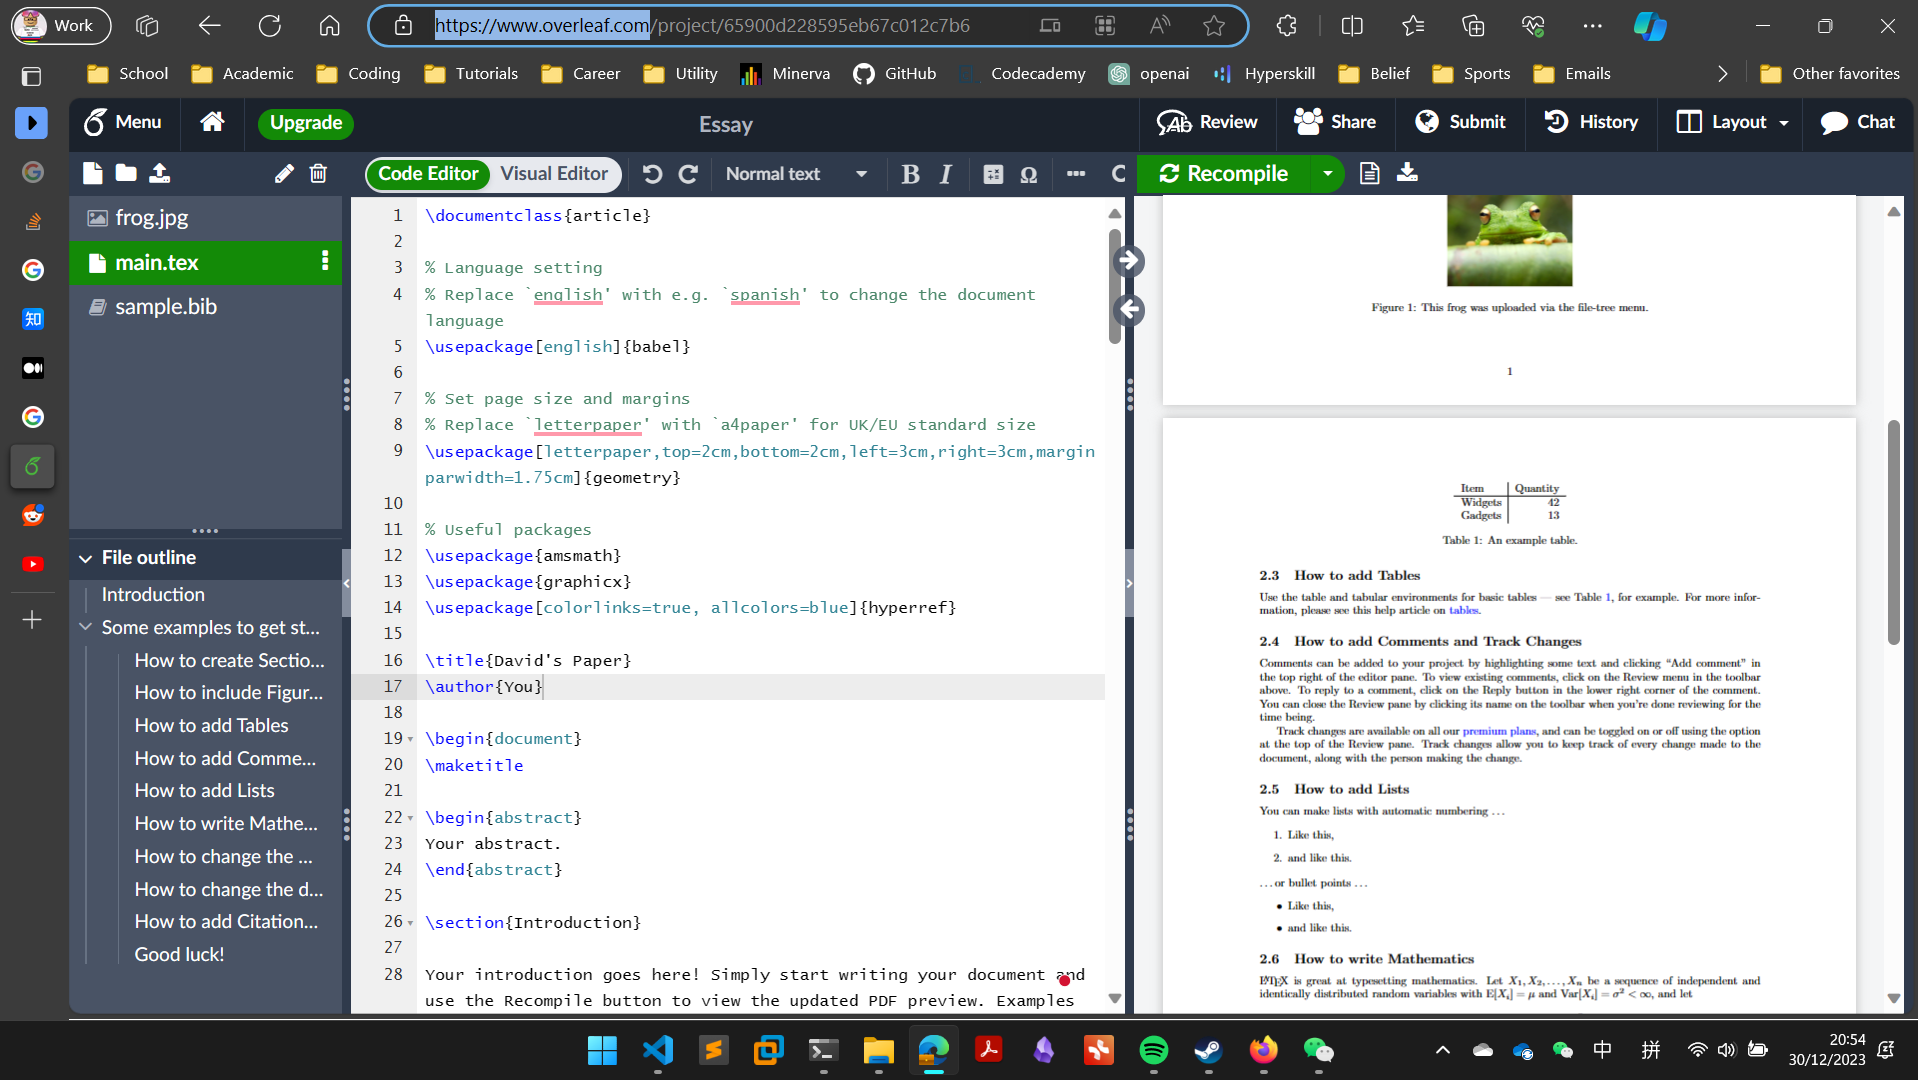
\includegraphics[width=0.25\linewidth]{test1.png}
\caption{\label{fig:frog}This frog was uploaded via the file-tree menu.}
\end{figure}

\subsection{How to add Tables}


Use the table and tabular environments for basic tables --- see Table~\ref{tab:widgets}, for example. For more information, please see this help article on \href{https://www.overleaf.com/learn/latex/tables}{tables}.

\begin{table}[h]
\centering
\begin{tabular}{l|r}
Item & Quantity \\\hline
Widgets & 42 \\
Gadgets & 13
\end{tabular}
\caption{\label{tab:widgets}An example table.}
\end{table}

\subsection{How to add Comments and Track Changes}

Comments can be added to your project by highlighting some text and clicking ``Add comment'' in the top right of the editor pane. To view existing comments, click on the Review menu in the toolbar above. To reply to a comment, click on the Reply button in the lower right corner of the comment. You can close the Review pane by clicking its name on the toolbar when you're done reviewing for the  being.

Track changes are available on all our \href{https://www.overleaf.com/user/subscription/plans}{premium plans}, and can be toggled on or off using the option at the top of the Review pane. Track changes allow you to keep track of every change made to the document, along with the person making the change.

\subsection{How to add Lists}

You can make lists with automatic numbering \dots

\begin{enumerate}
\item Like this,
\item and like this.
\end{enumerate}
\dots or bullet points \dots
\begin{itemize}
\item Like this,
\item and like this.
\end{itemize}

\subsection{How to write Mathematics}

\LaTeX{} is great at typesetting mathematics. Let $X_1, X_2, \ldots, X_n$ be a sequence of independent and identically distributed random variables with $\text{E}[X_i] = \mu$ and $\text{Var}[X_i] = \sigma^2 < \infty$, and let
\[S_n = \frac{X_1 + X_2 + \cdots + X_n}{n}
      = \frac{1}{n}\sum_{i}^{n} X_i\]
denote their mean. Then as $n$ approaches infinity, the random variables $\sqrt{n}(S_n - \mu)$ converge in distribution to a normal $\mathcal{N}(0, \sigma^2)$.


\subsection{How to change the margins and paper size}

Usually the template you're using will have the page margins and paper size set correctly for that use-case. For example, if you're using a journal article template provided by the journal publisher, that template will be formatted according to their requirements. In these cases, it's best not to alter the margins directly.

If however you're using a more general template, such as this one, and would like to alter the margins, a common way to do so is via the geometry package. You can find the geometry package loaded in the preamble at the top of this example file, and if you'd like to learn more about how to adjust the settings, please visit this help article on \href{https://www.overleaf.com/learn/latex/page_size_and_margins}{page size and margins}.

\subsection{How to change the document language and spell check settings}

Overleaf supports many different languages, including multiple different languages within one document.

To configure the document language, simply edit the option provided to the babel package in the preamble at the top of this example project. To learn more about the different options, please visit this help article on \href{https://www.overleaf.com/learn/latex/International_language_support}{international language support}.

To change the spell check language, simply open the Overleaf menu at the top left of the editor window, scroll down to the spell check setting, and adjust accordingly.

\subsection{How to add Citations and a References List}

You can simply upload a \verb|.bib| file containing your BibTeX entries, created with a tool such as JabRef. You can then cite entries from it, like this: \cite{greenwade93}. Just remember to specify a bibliography style, as well as the filename of the \verb|.bib|. You can find a \href{https://www.overleaf.com/help/97-how-to-include-a-bibliography-using-bibtex}{video tutorial here} to learn more about BibTeX.

If you have an \href{https://www.overleaf.com/user/subscription/plans}{upgraded account}, you can also import your Mendeley or Zotero library directly as a \verb|.bib| file, via the upload menu in the file-tree.

\subsection{Good luck!}

We hope you find Overleaf useful, and do take a look at our \href{https://www.overleaf.com/learn}{help library} for more tutorials and user guides! Please also let us know if you have any feedback using the Contact Us link at the bottom of the Overleaf menu --- or use the contact form at \url{https://www.overleaf.com/contact}.

\bibliographystyle{alpha}
\bibliography{sample}

\end{document}